% Document format
\documentclass[12pt,oneside]{memoir}
\usepackage[
    top=2.5cm, bottom=2.5cm, left=3.5cm, right=2.5cm,
    marginparwidth=0cm
]{geometry}
\renewcommand{\baselinestretch}{1.5}

\usepackage{fancyhdr}
\pagestyle{fancy}
\fancyhf[RH]{\thepage}
\fancyfoot{}

\usepackage{multicol}
\counterwithout{figure}{chapter}
\counterwithin*{equation}{section}
\usepackage{textcomp}
\raggedbottom

\renewcommand*{\cftchapterfont}{\normalfont}
\setsecnumdepth{subsection}

\usepackage[font=small,labelsep=period,labelfont=bf]{caption}

\usepackage{fontspec}
\linespread{1.5}

\usepackage{enumitem}
\usepackage{indentfirst}
\usepackage{graphicx}
\usepackage{float}
\usepackage{hyperref}
\usepackage{amsmath}
\usepackage[bottom]{footmisc}

% Chapter title formatting
\usepackage{titlesec}
\titleformat{\chapter}[display]
{\normalfont\huge\bfseries}{\chaptertitlename\ \thechapter}{-10pt}{\Large}
\titlespacing*{\chapter}{0pt}{-15pt}{0pt}
\assignpagestyle{\chapter}{fancy}

% Bibliography
\usepackage[
    backend=bibtex, style=authortitle, defernumbers=true,
]{biblatex}
\addbibresource{common/bibliography.bib}

% For each cited reference create a category named "cited"
\DeclareBibliographyCategory{cited}
\AtEveryCitekey{\addtocategory{cited}{\thefield{entrykey}}}

% Add rule for annotated bibliography
\DeclareFieldFormat{annotation}{
    \\ \indent{\textbf{Annotation:}\addspace #1}\\
}

\renewbibmacro*{finentry}{%
  \iffieldundef{annotation}
    {\finentry}
    {\setunit{\finentrypunct\par\vspace{\bibitemsep}\nobreak}
     \printfield{annotation}%
     \finentry}}


% Bibliography
\usepackage[
    backend=bibtex, style=authortitle, defernumbers=true,
]{biblatex}
\addbibresource{bibliography.bib}

% For each cited reference create a category named "cited"
\DeclareBibliographyCategory{cited}
\AtEveryCitekey{\addtocategory{cited}{\thefield{entrykey}}}

% Add rule for annotated bibliography
\DeclareFieldFormat{annotation}{
    \\ \indent{\textbf{Annotation:}\addspace #1}\\
}

\renewbibmacro*{finentry}{%
  \iffieldundef{annotation}
    {\finentry}
    {\setunit{\finentrypunct\par\vspace{\bibitemsep}\nobreak}
     \printfield{annotation}%
     \finentry}}

\begin{document}
\pagenumbering{gobble}

\begin{titlingpage}

\begin{figure}[H]
\vspace{-2cm}
\hspace{-2.5cm}

\includegraphics[scale=0.30]{common/images/header.png}
\end{figure}

\vfill

\begin{center}
\hspace{-0.5cm}
\Huge{\textbf{Language processing of a constructed \\language: the case of Lojban}}\\
\end{center}

\vfill


\begin{tabular}{b{6.5cm}b{7.5cm}}
\textsc{Madeira Cortes} André & Travail d'initiation à la recherche présenté sous la direction de Max \textsc{De Wilde}
en vue de l'obtention du titre de Master en Sciences et Technologies de l'Information et de la Communication\\
\end{tabular}

\vfill

\begin{center}
\Large Année académique 2021--2022
\end{center}

\end{titlingpage}

\newpage
\newgeometry{left=2.5cm, top=0.5cm, bottom=1cm}
\vspace{-1cm}
\setcounter{tocdepth}{3}
\tableofcontents*
\vspace{-1cm}
\listoffigures*
\restoregeometry
\newpage

\pagenumbering{arabic}
\chapter{Introductory chapter (draft)}

\vspace{0.5cm}

People have wondered for centuries how to improve languages in order to be more efficient, to communicate in an easier way, and with fewer ambiguities.
Most of the time, these questions surface when discussing how to disseminate information and research, notably in scientific fields, when a shared language
between two parties does not exist and a "lingua franca" is required. Thus started the search for an "universal" language.

\section{Universal language}

This line of inquiry is indeed far from being modern: for centuries, Jewish and Catholic scholars searched for the "Adamic language", under the belief that
all of humanity spoke the same language until the construction of the Tower of Babel and the fragmentation of human languages (an event called "confusio linguarum",
the confusion of tongues \footnote{Genesis 11:1-9}). In the seventeenth century, with the sharp decline of Latin as a shared language among scholars, a newfound interest in
the subject sparked since collaboration between researchers of different countries required many of them to become polyglots. While there was an obvious hegemony of the English,
German, and French languages as the "scientific languages" at the time, interest among all research fields in the knowledge from countries other than those in Central Europe grew.
Language had become a central factor (or even requirement) to acquire knowledge from authors across the world, and an "universal" language was becoming increasingly important to some.\newline

While discussing the various requirements needed to share one's knowledge with others, philosopher Francis Bacon posited in his 1605 book that some languages use what
he calls "characters real", allowing people which do not share a common oral language to understand each other in written form, which should be a goal when creating a
medium allowing researchers in the fields of science, philosophy and others to communicate:

\begin{quote}
    "(...) And we understand further, that it is the use of China and the kingdoms of the High Levant to write in characters real, which express neither letters nor words in gross, but
    things or notions; insomuch as countries and provinces which understand not one another’s language can nevertheless read one another’s writings, because the characters are accepted
    more generally than the languages do extend; and, therefore, they have a vast multitude of characters, as many, I suppose, as radical words."
    \footnote{\cite{bacon1605proficience} (the position of the quote depends on the various editions and publishing formats of the book, but most commonly found in Book II, Chapter XVI)}
\end{quote}

Other authors explored the same concept, most notably Leibniz and his "characteristica universalis", which according to him allowed users to express mathematical, scientific, and metaphysical
concepts. He wrote at length about it, creating a trove of pictograms and diagrams expressing complex notions (an example of which can be found in
"Dissertatio de arte combinatoria" \footnote{\cite{leibniz1666dissertatio}}).

\begin{figure}[H]
\centering
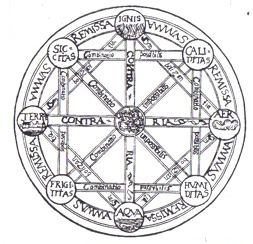
\includegraphics{images/characteristica_universalis_diagram.jpg}
\caption{Leibniz's diagrammatic reasoning in "Dissertatio de arte combinatoria"}
\end{figure}

\newpage
While these first forays into the subject solely wanted a language for scholars, more ambitious plans for an artificial language that all nations and people could use came soon after,
with scepticism from several authors. An example of such disagreement can be found in some of Descartes' letters exchanged with fellow polymath Marin Mersenne (in 1629), the former
stating that he does not see any use for such a language, but if it were to exist it would require several aspects:

\begin{itemize}
    \setlength\itemsep{-0.5em}
    \item be international;
    \item outlined by a simple grammar, which could be learned in a few hours;
    \item possess neither exceptions nor irregularities. \footnote{\cite[76-82]{descartes1897oeuvres}}
\end{itemize}

The disagreement notwithstanding, Mersenne eventually created his own "universal language for research" in his 1636 book "Harmonie universelle, contenant la th{\'e}orie et la pratique
de la musique", which contains a proposal for a "perfect language", expressing scientific concepts through music. \footnote{\cite[Book I, proposition 24]{mersenne1636}}

\section{Constructed languages}

The criteria defined by Descartes are still today the baseline that a lot of authors use for the definition of what an optimal language should be, and are at the core of many of the most
famous constructed languages in existence like Volapük and Esperanto. But what are constructed languages?\newline

(SMALL INTRO TO EXPLAIN WHAT CONSTRUCTED LANGUAGES ARE) \newline

For an in-depth history of constructed languages, I vividly recommend the reader to explore Arika Okrent's book "In the land of invented languages" \footnote{\cite{okrent2009land}} which,
while not being a scientific publication, is an extremely comprehensive and rich book to explore the subject.\newline

Albeit still being a niche subject, constructed languages have grown in popularity in the last few years. Following the popularity of Esperanto, which boasts a growing
number of speakers, a few constructed languages have risen to the eyes of the public given their origins. Most of these languages originate in works of fiction,
which in turn generate speakers due to the popularity of those same works of fiction. The most notable example of this growth in popularity is the language learning
platform "Duolingo" introducing courses for three such languages: Esperanto (the most famous and widespread constructed language ever), High Valyrian (invented for the TV show
"Game of Thrones") and Klingon (invented for the TV show "Star Trek"). \newline

Unfortunately, due to the stark difference in popularity between Esperanto and other constructed languages, research in the field of linguistics has mostly been focused in the former.
This focus is understandable, since Esperanto is one of the few constructed languages that can boast having native speakers. Detlev Blanke, in "Planned Languages - a Survey of some of the main Problems",
highlights this achievement, putting Esperanto in a category of its own as a full-fledged language, and not a "language project" or a "semilanguage". He theorises that it is the only constructed language
which has gone through nineteen evolutionary steps he describes, from the publication of its structure to the appearance of the first bilingual children \footnote{\cite{blanke1989planned}}. Since the publication
of this article, Klingon can probably claim the same status, but researchers probably don't delve into it as much due to its origins. Nonetheless, authors have been urging researchers to study other
constructed languages, as these may have troves of interesting linguistic elements \footnote{\cite{oostendorp2001constructed}}.

\section{Lojban}

\subsection{The roots: the history of Loglan}

The first constructed language whose main aim is optimality is most probably Loglan, introduced by James Cooke Brown and first published
in Scientific American \footnote{\cite{brown1960loglan}}. This is a notable achievement: rarely had a major scientific periodical devoted publishing
space to a constructed language other than Esperanto. This is probably due to the fact that Brown presented it with a purely scientific approach, and no big societal aims
(at first --- history will change that). Loglan, whose name is a contraction of the words "Logical" and "Language", was defined as having the following aims:

\begin{itemize}
    \setlength\itemsep{-0.5em}
    \item be purely based in logic;
    \item be culturally neutral;
    \item have a grammar small enough to be teachable, but complex enough to allow conversations;
    \item be unambiguous.
 \end{itemize}

The history of Loglan will take a strange path after its first publication. Given its publication in a major scientific journal, and a growing audience
asking him for more information, Brown requested a raise from his university, which was declined, and a government grant, which was also refused multiple times.
Insulted, he eventually resigned from his research position and, using money gathered by activities other than scientific research, started his own institute,
the "Loglan Institute". Later, in 1975, he published a book about the language. At the institute, he surrounded himself mostly by admirers, most of which were computer science
students and researchers who were excited by the possibility of the language serving as a human-computer interface. Thus, Brown rarely opened himself to critics,
which might have influenced the inflated sense of importance he felt Loglan had. A less explicit aim for the language, which was presented at a later point, was attempting
to prove the hypothesis of linguistic relativity (also known as the Sapir–Whorf hypothesis, or simply the Whorf hypothesis) in its strong version.
Most modern linguists would disagree with this statement, but Brown was convinced that the usage of Loglan would allow speakers to think more logically, and expand their
intelligence.\newline

With a growing audience, and the transformation of the institution into a "membership-controlled corporation" (in order to request paying fees to all the volunteers),
Brown started to see that its members wanted to steer his creation in a direction which he did not enjoy. Trying to remain in control, he fired most of the board.
This event and others created a schism in the Loglan community, and little by little a separatist group grew, which gave birth to Lojban.

\subsection{The creation of Lojban}

Starting in 1987, The Logical Language Group (LLG) worked to create a constructed language which aimed to extend the existing Loglan language and improve it further,
in order to make it easier to learn by humans and more readily accessible. This work culminated with the publication of a book in 1997 by
John Woldemar Conwan \footnote{\cite{cowan1997complete}}, an American programmer otherwise known for his work with XML and Unicode, among other things. This book is,
still today, considered the baseline of the language, defining its whole grammar, vocabulary, and semantics.\newline

Over the years, Brown disputed several times in court that this creation infringed his copyright. Several trials later, all courts agree that both projects are independent,
and Lojban took over Loglan in popularity and contributors.

\subsection{Brief introduction to the Lojban grammar}

Lojban sentences are constructed in a way that expresses a logical predicate, with a fixed set of arguments. For a small
refresher course in predicate logic see Annex A.\newline

The recurring "first approach to the language" example used in most Lojban literature, from the language standard to research papers
is the sentence "John is the father of Sam". In this sentence, there is a clear predicate ("is-the-father-of") and two arguments
("John" and "Sam").

\begin{figure}[H]
\centering
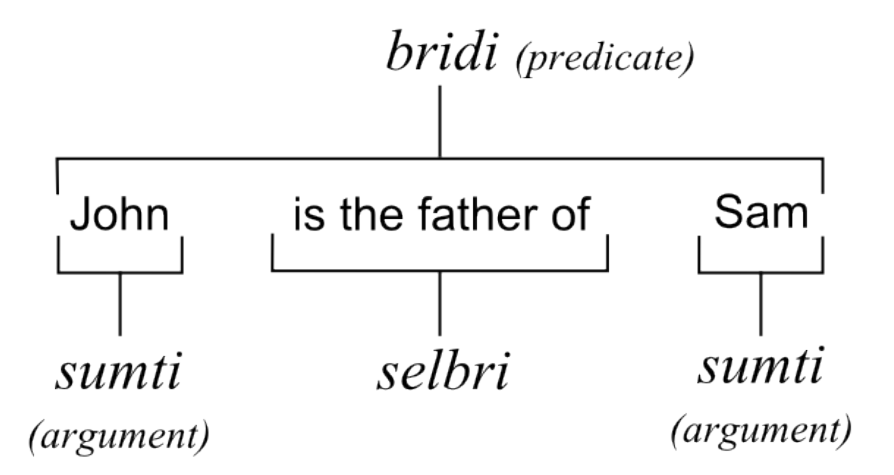
\includegraphics[scale=0.20]{images/lojban_grammar.png}
\caption{Basic structure of a Lojban sentence (Source: \cite{cowan1997complete})}
\end{figure}

This figure presents the three most important base elements of a sentence in Lojban:

\begin{itemize}
    \item \textbf{bridi}: the predicate expression
    \item \textbf{selbri}: the word(s) acting as the predicate
    \item \textbf{sumti}: positional argument passed to the predicate
\end{itemize}

Selbri are strictly defined by representations which position the sumti around a key word. For example, the selbri to describe the fatherhood relationship is "patfu":

$$\text{patfu}: x_1 \: \text{is a father of} \: x_2$$

Thus, the above sentence is expressed in Lojban as: \textbf{la .djon. patfu la .sam.} \newline

The position of the sumti is rigid and allows to release the sentence from any ambiguity. We always know who is the father and who is the child. Of course, in this example,
the English counterpart doesn't really make sense (the sentence "Sam is 'fathered' by John" makes absolutely no sense), but for a non-native speaker the order of words in
other pairs of sentences might add ambiguity. For example, a non-native might get confused about the difference between the sentences "John eats the bread" and "The bread is
eaten by John", as this construct does not exist in their language.\newline

Of course, this framework of predicate expressions is simply the base feature of the language, but many others allow it to cover the other missing aspects that most natural
languages feature: tenses, relative clauses, abstractions, emotional indicators, and others. These will be explored in a further chapter in the thesis. \newline

\section{What this thesis aims to achieve}

At its root, computer science had a singular aim --- automating calculations for a broad spectrum of use-cases. However with time and with the emergence of better, faster, and
stronger computers, researchers understood that computers could be used to achieve far more complex tasks. Several diverse research fields made their appearance, and among these
some realised that computing could help us structure the flow of information, in addition to making calculations based on it. \newline

The explosion of tasks requiring the processing of large amounts of structured data inside of companies, and much later the arrival of the Internet, forced us to debate and
research subjects such as: how to gather information, how to manage and store it, analyse and interpret it, explore it, etc... A sizeable chunk of this information comes to us
in the form of text and language, in their many forms. To answer these needs, language engineering became a central research field in a new society, one which had migrated
from a purely industrial society to an "information society".\newline

The main aim of this thesis is to explore the intersection between the two fields presented in this introduction: linguistics, around the subject of a particular constructed
language, and computer science, which allows language processing. The first objective of this thesis is to outline the state of the art and existing parsers for Lojban, list both
their flaws and positive aspects, and define what kind of new parser would be interesting to develop. Using the Python programming language, one such parser will be created, including
also a way to visualise the structure of the sentences parsed, in order to analyse them.\newline

If possible, a secondary objective would be to create a minimal proof of concept of machine translation using Lojban as an interlingua between English and French. This type of translation
method would of course never challenge existing models, which are based on artificial intelligence and have shown incredible results that never cease to improve. However, it is an interesting
research prototype: Lojban claims to be a syntactically unambiguous language which improves human-human communication but also human-computer communication. While the former is more complicated
to prove, since the amount of speakers of Lojban around the world is not immense, the latter has been studied. Research has already postulated that Lojban (or variants of it) would be interesting
interlinguas between humans and computers \footnote{\cite{speer2004meeting}} or artificial intelligences \footnote{\cite{goertzel2013lojban}}.

\chapter{Table of contents draft}
\label{chap:draft_toc}

\begin{enumerate}
    %\setlength\itemsep{-0.4em}
    \item \textbf{Introduction} (see Chapter 1 for a first draft of this introductory chapter)
        \vspace{-0.4cm}
        \begin{enumerate}[label*=\arabic*.]
            \setlength\itemsep{-0.5em}
            \item \textbf{Universal language}
            \item \textbf{Constructed languages}
            \item \textbf{Lojban}
            \vspace{-0.4cm}
            \begin{enumerate}[label*=\arabic*.]
                \setlength\itemsep{-0.5em}
                \item \textbf{The roots: the history of Loglan}
                \item \textbf{The creation of Lojban}
                \item \textbf{Brief introduction to the Lojban grammar}
            \end{enumerate}
            \item \textbf{What this thesis aims to achieve}
        \end{enumerate}
    \item \textbf{State of the art}
        \vspace{-0.4cm}
        \begin{enumerate}[label*=\arabic*.]
            %\setlength\itemsep{-0.5em}
            \item \textbf{Existing research} (brief analysis of existing research on language parsers in general, and Lojban specifically)
            \item \textbf{Existing resources} (brief overview of tools, resources, and software that exists around the language)
        \end{enumerate}
    \item \textbf{Longer introduction to the Lojban grammar} (required to understand the following chapters and how the parser will be constructed)
    \item \textbf{Parsing of Lojban sentences}
        \vspace{-0.4cm}
        \begin{enumerate}[label*=\arabic*.]
            %\setlength\itemsep{-0.5em}
            \item \textbf{Description of the created library} (writing code which parses a Lojban sentence and creates, using formal logic, a framework to understand the sentence based on the Lojban grammar)
            \item \textbf{Examples} (showing examples of the generated logical framework and how it effectively describes the Lojban sentence)
        \end{enumerate}
    \item \textbf{Deducing meaning from a parsed sentence}
        \vspace{-0.4cm}
        \begin{enumerate}[label*=\arabic*.]
            %\setlength\itemsep{-0.5em}
            \item \textbf{Description of the created library} (drawing upon the code written and outlined in the previous chapter, attempting to translate the Lojban sentence into a sensible sentence in English using a dictionary)
            \item \textbf{Examples} (showing examples of translations achieved with the program written)
        \end{enumerate}
    \item \textbf{Using Lojban as an interlingua} (small attempts, with a limited corpus, of creating a system of basic machine translation using Lojban as an interlingua)
    \item \textbf{Conclusions}
    \item \textbf{Bibliography}
    \item \textbf{Annex A - Predicate Logic} (small annex giving an introduction to predicate logic, in case the readers need a refresher to understand the basis of the Lojban grammar)
\end{enumerate}

\chapter{Thesis Work Plan}

\section{Deadlines}
\label{sec:deadlines}

The following broad outline is what I imagine, if possible, to be the list of big
deadlines for the academic year in which the thesis will be written:

\begin{itemize}
    \vspace{-0.4cm}
    \item \textbf{Status meetings:} Depending on the availability of the thesis director,
    I'd suggest holding these meetings (or emails) every month and a half to discuss advances
    on the thesis. For example, meetings in mid-October 2022, end of November 2022, mid-January 2023,
    end of February 2023 and mid-April 2023.
    \item \textbf{Final delivery:} Around May 2023.
    \item \textbf{Final presentation:} Around June 2023.
\end{itemize}

\vspace{-0.8cm}

\section{Organizing work}
\label{sec:organizing_work}

Given my background in IT, and as a software developer by profession, I would like
to organise my work for this Master Thesis as I'm used to: like a software project.
I'm planning to version the thesis \LaTeX \ document in a version control system
(most probably Git using Github). This allows to backup the document gradually,
as well as providing a better method to track the evolution of the document.\newline

I am also envisioning to write a "Changelog" file during the elaboration of the
thesis, and presenting it during the "status meetings" with the thesis director, as described above.
This allows for a better understanding of what changed between two versions of the thesis,
instead of having to read it in its entirety each time.


% Bibliography

\nocite{*}
\renewcommand{\bibname}{Annotated Bibliography}
\printbibheading
\printbibliography[
    category=cited,
    heading=subbibliography,
    title={Cited in the introduction draft},
    resetnumbers
]
\newpage
\printbibliography[
    notcategory=cited,
    heading=subbibliography,
    title={Further reading for the thesis},
    resetnumbers
]

\end{document}
